\documentclass[12pt]{article}
\usepackage[margin=1in]{geometry}
\usepackage{natbib}
\usepackage{graphicx}
\usepackage{caption}
\usepackage{subcaption}
\usepackage{multirow}
\usepackage{longtable}
\usepackage{color}
\bibliographystyle{apalike}

\begin{document}

\title{Evolutionary genomics of peach \\and almond domestication}

\author{\small\sfbf{Dianne Velasco$^{\S}$, Mallikarjuna Aradhya$^{\dag}$, Jeffrey Ross-Ibarra$^{\S\ddag}$}\thanks{Corresponding author: Department of Plant Sciences, University of California, Davis, California 95616, USA. E-mail: \mbox{rossibarra@ucdavis.edu}} \\[0.3cm]
     \small\sf $^{\S}$Department of Plant Sciences, University of California, Davis, California 95616, USA,\\
     \small\sf $^{\dag}$USDA-ARS National Clonal Germplasm Repository, Davis, California 95616, USA,\\
     \small\sf $^{\ddag}$Center for Population Biology and Genome Center, University of California, Davis, California 95616, USA}

\date{\today}

\maketitle

\section*{Introduction}
\emph{Prunus} is the largest genus in the family Rosaceae with approximately four hundred species including multiple domesticated crops (almond, apricot, cherry, peach, and plum) in three of its five subgenera.
%reference to number of approximate number of species, number depends on reference
%
The subgenus \emph{Amygdalus} includes the most morphologically distinct sibling species, \emph{P. persica} (Mill.) D. A. Webb (peach) and \emph{P. dulcis} (L.) Batsch (almond).
%NOTE: somehow want to include that the species are interfertile, or somehow indicate how similar they are
%
While \emph{Prunus} species are generally outcrossing due to gametophytic self-incompatibility, though self-compatible alleles are known to exist in multiple species across the genus, peach is fully self-compatible. 
%
Domestication of almond and peach occurred approximately 5000 years ago in the Fertile Crescent and China \citep{zohary2012domestication}, respectively, followed by global dissemination \citep{hedrick1917peaches, edwards1975almond, gradziel2011origin, zheng2014archaeological}.
%
Both domestication and mating system have been shown to significantly impact genome evolution in annual species \citep{glemin2006impact, doebley2006molecular, slotte2013capsella}. 
%
However, the manner in which domestication and mating system influence genome evolution of tree species remains poorly understood \citep{mckey2010evolutionary}.
\\
\\
%BACKGROUND ON SPECIES
%
In addition to having a similar length of domestication, peach and almond are also similar in early fruit development, perenniality, precocity, genome organization \citep{arus2012peach}, and genome size \citep{arumuganathan1991nuclear, dickson1992nuclear, baird1994estimating,  loureiro2007two}.
%
Most striking however are their obvious differences in mature fruit morphology and mating systems, but almond and peach also differ in life span (longer v. shorter), chilling requirements (lower v. higher) and adventitious root generation (poor v. good).
%
The few obvious traits associated with domestication in almond are reduced toxicity, thinner endocarp, and increased seed size, while domestication traits in peach are characterized by diverse fruit morphology (size, color, texture, shape, etc.) and self-compatibility.
%
However, other traits associated with both almond and peach, such as precocity, or solely with peach, such as relative ease of adventitious rooting, may have also been targeted or incidentally selected during domestication. 
%
Unfortunately, efforts to determine species relationships within the subgenus and identify wild progenitors of almond and peach \citep{verde2013high, aradhya2004molecular, zeinalabedini2010origin, mowrey1990isozyme, browicz1996genus, ladizinsky1999origin, bassi20081} have had mixed results. 
%
Given the uncertainty identifying wild progenitors of almond and peach, domestication studies using crossing experiments are particularly difficult in addition to being generally impractical with long-lived perennial species.
%citation for crossing experiments doesn't quite seem to fit, perhaps one of Doebley's papers or others using domesticated x wild cross to identify loci
%
\\
\\
Peach and almond are both diploid with a haploid chromosome number of eight, as are all species within the subgenus \emph{Amygdalus}, and genetic mapping from an almond x peach F2 population suggests they have a similar genomic structure \citep{dirlewanger2004comparative}. 
%
At 220-230 Megabases (Mb) the recently sequenced peach genome \citep{verde2013high} is less than double the genome size of model plant \emph{Arabidopsis thaliana}.
%
The genome size of almond is also relatively, estimated at  nearly 300 Mb, similar to pre-sequencing estimates for peach \citep{arumuganathan1991nuclear}. 
%
The small genome size and chromosome number of peach and almond support their use as a model to investigate the effects of domestication and mating system in trees.
%
\\
\\
%DOMESTICATION VERSUS SI/SC IN GENOME
Domestication reduces diversity at multiple loci throughout the genome \citep{glemin2006impact, doebley2006molecular, slotte2013capsella} while self-fertilization reduces diversity across the entire genome.
%
The mating system of a species affects its genome evolution, and studies in closely related species pairs with alternate mating systems, such as \emph{Arabidopsis thaliana} and \emph{A. lyrata} and \emph{Capsella rubella} and \emph{C. grandiflora} \citep{slotte2013capsella}, have enabled investigation of this phenomenon. 
%
These analyses reveal that mating system has a significant effect on nucleotide diversity, linkage disequilibrium (LD), heterozygosity, genome size, repeat content, and genetic load. 
%
As both species have undergone domestication bottlenecks, the expectation is that localized reductions in genomic diversity are due to selection, but widespread differences in genomic diversity are likely due to alternate mating systems \citep{glemin2006impact, charlesworth2001breeding}. 
%
Loci selected during or subsequent to domestication should be evidenced by reduced localized genomic diversity.
%
lower genome-wide diversity in the self-compatible peach compared to the self-incompatible almond.
%
%Domestication in plants is associated with changes in many traits, such as increased size and morphological diversity of the harvested organ (seed, fruit, leaves, etc.), reduced seed dispersal, adaptation to disturbed environments, reduced toxicity, selfing, photoperiod insensitivity, etc. \citep{doebley2006molecular}, but a relative few of these changes are striking in almond or peach. 
%seed size in almond, fruit size & color in peach
%range of bloom/maturity dates for peach
%sweet kernels in almond
%what about other tree crops?
%
\\
\\
%STUDY PURPOSE AND SUMMARY
Resequencing several diverse almond genomes and publicly available resequenced peach genomes for comparative analysis. 
%
Seek to understand how domestication and mating system affect the genome evolution of closely related species with alternate mating compatibility
%
Almond and peach are both highly valued crops, but peach serves as a model system for Prunus and tree crops in general due to its small genome (230 Mb), short generation time (2-3 years), and self-compatibility \citep{arus2012peach}.
%
The recently sequenced peach genome \citep{verde2013high}serves as a reference genome for the genus, but the primary peach genetic map is based on an almond x peach F2 population \citep{arus2012peach, joobeur1998construction, aranzana2003set, dirlewanger2004comparative, dominguez2003plant}.
%
However, genomic sequence data provides a way to begin investigating domestication with a lower difficulty threshold.
%
Recent analysis of resequenced peach genomes indicates low genetic diversity and higher LD across the genome compared to wild peach species \citep{verde2013high}. 
%
%However, without sequenced almond genomes, the same information is not known for almond, and expectations are that due to self-incompatibility it will have higher levels of heterozygosity and lower LD compared to peach.
%
Understanding how domestication and mating systems may have contributed to genome evolution in almond and peach expands the understanding of these processes beyond annual species. 
%
By identifying candidate domestication loci this study also provides an opportunity to determine which loci in almond and peach were under selection and whether common loci have similar or differing haplotypes. 
%
It also allows us to investigate if there are loci not typically found in domestication studies of annual crops. 
%
Mating system analysis of almond and peach expands the basic understanding of genome evolution in perennial species. 
%
Knowledge gained from these analyses provides valuable information regarding domestication loci and haplotypes, an
important resource for tree breeding programs.
%
The peach and almond will provide a model for evolution and domestication in tree species.
\\
\\
\section*{Materials and Methods}
%
\subsection*{Samples}
Resequenced genomes of domesticated species \emph{P. dulcis} and \emph{P. persica}, fourteen and thirty-two respectively, and one each of closely related species, \emph{P. fenzliana} and \emph{P. ferganensis}, and plum outgroup, \emph{P. cerasifera} were used for analysis.
%
Of the fourteen resequenced \emph{P. dulcis} genomes, five were from public sources (four from \citealt{koepke2013comparative}(?) via NCBI SRA and one RosBREED) and nine were newly resequenced samples (one at BGI and eight at UC Berkeley).
%
Thirty-one of thirty-two \emph{P. persica} resequenced samples were from public sources (ten from \citealt{verde2013high} via NCBI SRA, three from \citealt{ahmad2011whole} via NCBI SRA and eighteen from RosBREED FTP site),
%probably removing due to low coverage (1-3X); may be good for other analysis
and one newly resequenced (at BGI).
%
The wild almond species, \emph{P. fenzliana}, and outgroup plum species, \emph{P. cerasifera}, were resequenced with this study (at BGI), while the wild peach species, \emph{P. ferganensis}, was publicly available from NCBI SRA \citep{verde2013high}.\\
%
%
\subsection*{Analysis}
\emph{Sequencing, Quality Control, and Mapping}\\
Newly resequenced samples in this study were sequenced as paired end at 100 bp read length. 
% Include details of library preparation?
%
All publicly available resequenced samples were paired end but varied in length from 80 to 100 bp in read length. 
% recheck this range
%
Regardless of source all FASTQ files were trimmed of remnant adapter sequences using Scythe and then further trimmed using base quality with Sickle. 
%
% Buffalo V: Scythe. [https://github.com/vsbuffalo/scythe]
% figure out citation for Scythe; include version
%
% Najoshi :Sickle [github.com/najoshi/sickle]
% same as for Scythe
%
Trimmed reads were then aligned to the peach v 1.0 reference using BWA-MEM using a minimum seed length of 10 and internal seed length of 28.5.
% using -k 10 -r 2.85 parameters
% -k INT		minimum seed length [19]
% -r FLOAT	look for internal seeds inside a seed longer than {-k} * FLOAT [1.5]
% internal seed length remains the same as default parameters
% picked this up from P. Morrell
%
 \citep{li2013aligning}. 
% bwa mem -k 10 -r 2.85
% provide explanation of parameters
%
Depth and alignment from SAMtools using depth and flagstat subprograms \citep{li2009sequence} 
determined a mean mapped sequence depth of 21.759, which ranged from 4.715 to 41.105 (supp. Figure \ref{fig:depth}).\\
%BQ20: mean 27.212, range 7.169 to 48.039 \\
%BQ20MQ20: mean 22.29, range 4.948 to 41.552\\
%BQ20MQ30: mean 21.759, range 4.715 to 41.105\\
%Should this be in Results section instead?
%
%several custom scripts (deposit to github repo, add URL) were used for initial processing of data or to extract data for downstream use\\
\\
\emph{SNP calling}\\ %If going this route
%
SNP calling using SAMtools pileup and BCFtools \citep{li2009sequence} \\
% may change to ANGSD
%
PopBAM analysis: SAMtools was used to merge bams and add new header \citep{li2009sequence} with appropriate sample and population information for use in PopBAM \citep{garrigan2013popbam}. SNPs called in PopBAM were output in the SweepFinder \citep{nielsen2005genomic} format and then analyzed.\\
% if not switching to ANGSD
%
\\
\emph{Locating/Identifying Sweeps}\\
%
%\citep{li2009sequence} %SAM format and SAMtools
%R
\\
%
\\
\emph{Loci of Interest}\\
%
\\
\emph{Species Comparisons}\\
%
%
\begin{center}
\begin{longtable}{lllll}
\caption[P. dulcis, P. persica and related species used in analysis.]{\emph{P. dulcis}, \emph{P. persica} and related species used in analysis.} \label{my-label} \\
\hline \hline \multicolumn{1}{l}{\textbf{Species}} &
\multicolumn{1}{l}{\textbf{Number}} &
\multicolumn{1}{l}{\textbf{Source}} &
\multicolumn{1}{l}{\textbf{Reference}}\\ \hline 
\endfirsthead

\multicolumn{4}{r}{{\bfseries \tablename\ \thetable{} -- continued from previous page}} \\
\hline \multicolumn{1}{l}{\textbf{Species}} &
\multicolumn{1}{l}{\textbf{Number}} &
\multicolumn{1}{l}{\textbf{Source}} &
\multicolumn{1}{}{\textbf{Reference}} \\ \hline 
\endhead

\hline \multicolumn{4}{r}{{Continued on next page}} \\ \hline
\endfoot

\hline \hline
\endlastfoot

                 %\multicolumn{4}{l}
                  \emph{P. dulcis} &4 &NCBI SRA &\citealt{koepke2013comparative}\\
                  \emph{P. dulcis} &1 &RosBREED &URL\\
                  \emph{P. dulcis} &8 &UC Berkeley &this study \\
                  \emph{P. dulcis} &1 &BGI &this study\\
                 %\multicolumn{4}{l}
                  \emph{P. persica} &10 &NCBI SRA &\citealt{verde2013high} \\ % format italics
                  \emph{P. persica} &3 &NCBI SRA &\citealt{ahmad2011whole} \\ % format italics
                  \emph{P. persica} &18 &RosBREED &URL \\ % format italics
                  \emph{P. persica} &1 &BGI &this study \\ % format italics
                 %Almond Board resequencing (performed at BGI)
                 \emph{P. fenzliana} &1 &BGI &this study\\
                 %UCD,ABC
                 \emph{P. ferganensis} &1 &NCBI SRA &\citealt{verde2013high}\\
                 \emph{P. cerasifera} &1 &BGI &this study\\ \hline
                 %outgroup
                 %NCBI SRA
               %note that the SRR IDs are from NCBI SRA
               %GDR/RosBREED (ftp://ftp.bioinfo.wsu.edu/species/Prunus_persica/RosBREED_Illumina/)

\end{longtable}
\end{center}


%add indicator whether sample was plant material or public sequence (reference does give some indication or possibly just put indication that when "this study" is the reference that it indicates that plant material was used)




\section*{Results}


\section*{Discussion}

\pagebreak
%\bibliographystyle{apalike} %can use here and not in header
\bibliography{references.bib}
%
%FIGURE EXAMPLE
%demographic effects (Figure \ref{fig:peach}) can impact deleterious allele distro
%
%SUBSCRIPT EXAMPLE
%$V_a$ influenced by demography\\
%
\pagebreak
\begin{figure}[b]
\centering
   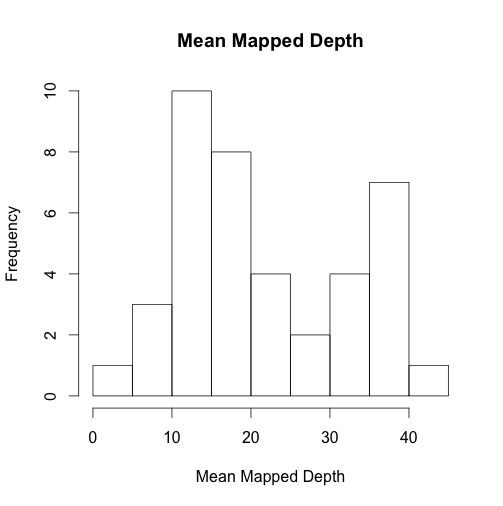
\includegraphics[width=0.8\textwidth]{depthBQ20MQ30.png}
  \caption{Mean mapped depth of sequenced used in analysis}
  \label{fig:depth}
\end{figure}

\begin{figure}[b]
\centering
   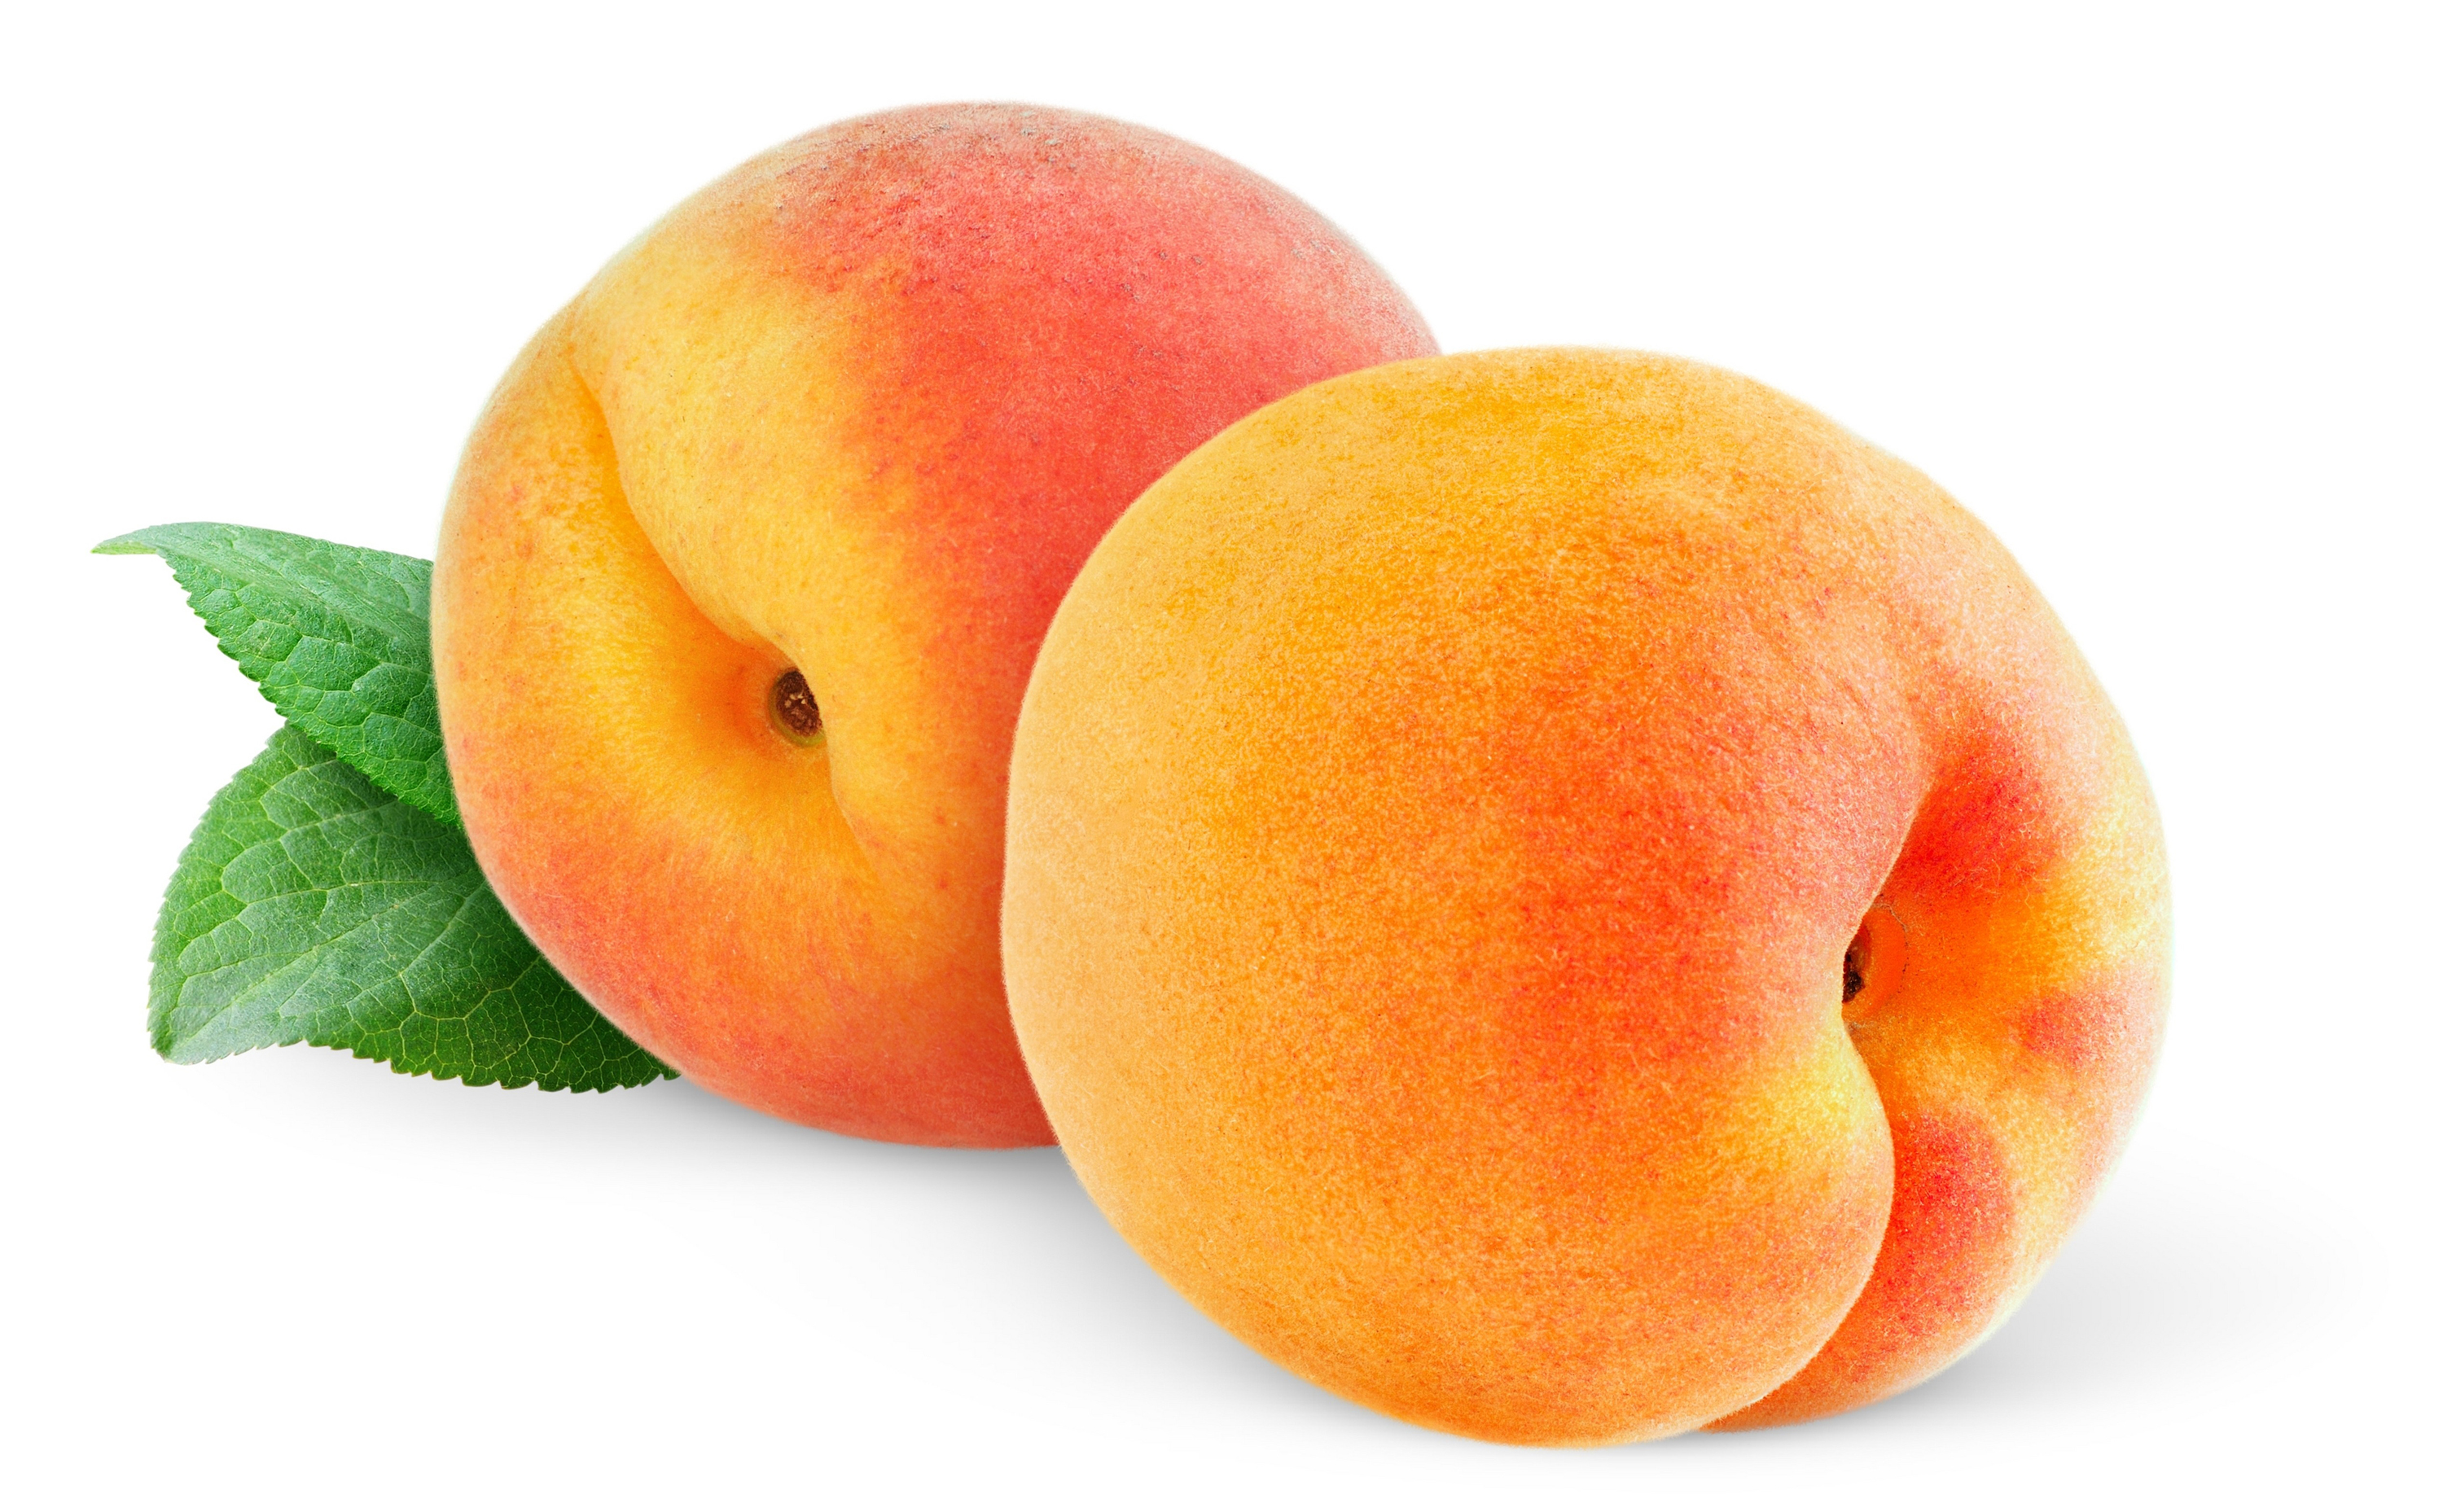
\includegraphics[width=0.8\textwidth]{peachzdfgad.jpg}
  \caption{Delicious peaches although the really new stuff in the paper will be about almonds}
  \label{fig:peach}
\end{figure}
%
\pagebreak
\section*{Supplementary Data}
%somehow change table number also maker table width match full width of text
\begin{center}
\begin{longtable}{lllll}
\caption[P. dulcis, P. persica and related species used in analysis.]{P. dulcis, P. persica and related species used in analysis.} \label{my-label} \\
\hline \hline \multicolumn{1}{l}{\textbf{Sample ID}} &
\multicolumn{1}{l}{\textbf{Accession and/or Cultivar}} &
\multicolumn{1}{l}{\textbf{Origin}} &
\multicolumn{1}{l}{\textbf{Source}}  &
\multicolumn{1}{l}{\textbf{Reference}} \\ \hline 
\endfirsthead

\multicolumn{5}{r}{{\bfseries \tablename\ \thetable{} -- continued from previous page}} \\
\hline \multicolumn{1}{l}{\textbf{Sample ID}} &
\multicolumn{1}{l}{\textbf{Accession and/or Cultivar}} &
\multicolumn{1}{l}{\textbf{Origin}} &
\multicolumn{1}{l}{\textbf{Source}} &
\multicolumn{1}{}{\textbf{Reference}} \\ \hline 
\endhead

\hline \multicolumn{5}{r}{{Continued on next page}} \\ \hline
\endfoot

\hline \hline
\endlastfoot

                 \multicolumn{5}{l}{\emph{P. dulcis}}  \\
%		 PD01 &DPRU 2578.2 & &NCGR &this study\\
		%Almond Board resequencing (BGI)
		% Not included because it appears to be possible F1 of peach x almond (or reverse)
                 PD02 &‘Tardy Nonpareil’ &USA &UCD &this study\\
		%Almond Board resequencing (BGI)
                 PD03 &DPRU 1791.3, BE-1609 &Turkey &NCGR &this study\\
		%Jastro resequencing (performed at UC Berkeley)
                 PD04 &DPRU 2374.12 &Iran &NCGR &this study\\
		%Jastro resequencing (performed at UC Berkeley)
                 PD05 &DPRU 1456.4, Badam &Pakistan &NCGR &this study\\
		%Jastro resequencing (performed at UC Berkeley)
                 PD06 &DPRU 2301, Tuono &Italy &NCGR &this study\\
		%Jastro resequencing (performed at UC Berkeley)
                 PD07 &DPRU 1462.2 &Pakistan &NCGR &this study\\
		%Jastro resequencing (performed at UC Berkeley)
                 PD08 &DPRU 1207.2 &Uzbekistan &NCGR &this study\\
		%Jastro resequencing (performed at UC Berkeley)
                 PD09 &DPRU 2331.9 &China &NCGR &this study\\
		%Jastro resequencing (performed at UC Berkeley)
                 PD10 &DPRU 0210, Languedoc &France &NCGR &this study\\ %Jastro resequencing (performed at UC Berkeley)
                 PD11 &S3067 &Spain &SRR765861 &\citealt{koepke2013comparative}?\\
		% resequenced at WSU by Amit Dhingra
                 PD12 &D05-187 &Spain &SRR765850 &\citealt{koepke2013comparative}?\\
		% resequenced at WSU by Amit Dhingra
                 PD13 &Lauranne &Spain &SRR765838 &\citealt{koepke2013comparative}?\\
		% resequenced at WSU by Amit Dhingra
                 PD14 &Ramillete &Spain &SRR765679 &\citealt{koepke2013comparative}?\\
		% resequenced at WSU by Amit Dhingra
                 PD15 &Nonpareil & USA&RosBREED &URL \\
                 \\
                 \multicolumn{5}{l}{\emph{P. persica}}  \\ % format italics
                 %PP01 &Lovell &USA &SRR502985 &\citealt{verde2013high}\\
                 % resequenced doubled haploid
                 PP02 &Yumyeong &Korea &SRR502994 &\citealt{verde2013high}\\
                 PP03 &Shenzhou Mitao&N China &
		\multirow{2}{1cm}{SRR502993, SRR502992} &\citealt{verde2013high}\\
                 %honey peach
                 \\
                 PP04 &Sahua Hong Pantao &S China &
		\multirow{2}{1cm}{SRR502991, SRR502990} &\citealt{verde2013high}\\
                 %flat peach
                 \\
                 PP05 &Quetta &Pakistan &
		\multirow{2}{1cm}{SRR502989, SRR502987} &\citealt{verde2013high}\\
                 \\
                 PP06 &Oro A &Brazil &SRR502986 &\citealt{verde2013high}\\
		%
                 PP07 &IF7310828 &Italy &
		\multirow{2}{1cm}{SRR503001, SRR503000} &\citealt{verde2013high}\\
                 \\
                 PP08 &GF305 &France &SRR502983 &\citealt{verde2013high}\\
                 PP09 &$F_1$ Contender $\times$ Ambra &Italy &SRR502997 &\citealt{verde2013high}\\
                 % peach x nectarine both P. persica
                 PP10 &Earligold &USA &
		\multirow{2}{1cm}{SRR502996, SRR502995} &\citealt{verde2013high}\\
                 \\
                 PP11 &Bolero &Italy &SRR501836 &\citealt{verde2013high}\\
                 PP12 &F8,1-42 &USA &SRR068361 &\citealt{ahmad2011whole} \\
                 PP13 &Georgia Belle &USA &SRR068359 &\citealt{ahmad2011whole} \\
                 PP14 &Dr. Davis &USA &SRR068360 &\citealt{ahmad2011whole} \\
                 PP15 &Lovell &USA &UCD &this study\\
                 % originally a canning variety selected ~1882
		% currently used as rootstock and/or control for disease screening
                 % FPS, ABC
                 % duplicate cultivar, BGI sequenced at higher depth
                 PP16 &DPRU 1190, Admiral Dewey&USA &RosBREED &URL \\
                 %aka PI 673525; introduced 1899
                 PP17 &Babcock &USA &RosBREED &URL \\
                 %introduced 1897
                 PP18 &Bolinha &Brazil &RosBREED &URL \\
		% released 1985
		% parentage: prob OP Aldrighi (Raseira et al. 1992; http://hortsci.ashspublications.org/content/27/11/1154.full.pdf)
		%considered resistant to brown rot (Monilinia fructicola); low chill
                 PP19 &DPRU 2142, Carman &USA &RosBREED &URL \\
		%Planted 1889 from OP seed (unknown variety) by J. W. Stubenrauch, Mexia, TX
		% data entry error listed as Carmen in GRIN; PI book has Carman
		% http://sun.ars-grin.gov:8080/npgs_public/prodweb.pdf0?in_vol=33&in_suffix=&in_page=052
                 %PI 673586; cultivar original PI 34673 assigned 1912
                 PP20 &Chinese Cling&China &RosBREED &URL \\
                 %introduced 1850; founder several cultivars
                 PP21 &Diamante&Brazil &RosBREED &URL \\
                 %predominant canning cultivar in Brazil per Okie (year & pub TBD)
                 PP22 &Dixon&USA &RosBREED &URL \\
		% Introduced in 1956
		% http://www.google.com/patents/USPP13911
		% early cling peach
                 %PP23 &Dr. Davis& &RosBREED &URL \\
                 % duplicate cultivar
                 PP24 &DPRU 0589, Early Crawford &USA &RosBREED &URL \\
                 %introduced before 1832
                 PP25 &Elberta&USA &RosBREED &URL \\
                 %introduced ~1889; OP sdlg of 'Chinese Cling’
                 PP26 &Florida Prince P138&USA &RosBREED &URL \\
                 %low chill cultivar; introduced in 2009
                 %PP27 &Georgia Bell&USA &RosBREED &URL \\
                 %(aka ‘Georgia Belle’ and ‘Belle of Georgia’
		% introduced ~1875; OP sdlg of Chinese Cling)
                 %not downloaded
                 %duplicate cultivar
                 PP28 &JH Hale&USA &RosBREED &URL \\
                 %male sterile; introduced 1912
                 %PP29 &Lovell &USA &RosBREED &URL \\
                 PP30 &Mayflower&USA &RosBREED &URL \\
                 %introduced 1909
                 %not yet downloaded
                 PP31 &Nemaguard &USA &RosBREED &URL \\
                 %rootstock; rumored to have P. davidiana in pedigree
                 PP32 &O'Henry &USA &RosBREED &URL \\
               %CODE FOR APOSTROPHE
                 %plant patent 2.964 1/27/1970; OP sdlg Merrill Bonanza; discovered 1960
                 PP33 &Okinawa &Japan &RosBREED &URL \\
		% Sharpe 1957
		% http://fshs.org/proceedings-o/1957-vol-70/320-322%20%28SHARPE%29.pdf
		% from 1953 seed lot, different seedlings
		%unsure if only one of these is what is now called 'Okinawa'
		% has nematode resistance
		% used in hybrid combination with Harrow's Blood (F2s) as rootstock
                 PP34 &Oldmixon Free &USA &RosBREED &URL \\
                 % introduced 1832
                 %not yet downloaded
                 PP35 &Rio Oso Gem &USA &RosBREED &URL \\
                 % introduced 1933
		% developed in Rio Oso, California, Sierra Nevada foothills
		% https://www.slowfoodusa.org/ark-item/rio-oso-gem-peach
                 PP36 &DPRU 2179, Slappey &USA &RosBREED &URL \\
                 %aka ‘Slappy’ in GRIN; introduced 1903
                 PP37 &DPRU 0941, St. John Yellow &USA &RosBREED &URL \\
                 %introduced 1860s
                 %some variety history at http://gapeaches.org/about-us/father-of-the-ga-peach-industry/
		\\
                 \multicolumn{5}{l}{Other \emph{Prunus} species}  \\
                 %Almond Board resequencing (performed at BGI)
                 PF01 &\emph{P. fenzliana} &? &UCD &this study\\
                 %UCD,ABC
                 PG01 &\emph{P. ferganensis} &Fergana Valley &
		\multirow{2}{1cm}{SRR502999, SRR502998} &\citealt{verde2013high}\\
                 \\
                 PC01 &\emph{P. cerasifera} DPRU 0579, Myrobalan &USA &NCGR &this study\\ \hline
                 %outgroup
                 %NCBI SRA
               %note that the SRR IDs are from NCBI SRA
               %GDR/RosBREED (ftp://ftp.bioinfo.wsu.edu/species/Prunus_persica/RosBREED_Illumina/)

\end{longtable}
\end{center}

\end{document}
